\chapter{Specifikacija programske potpore}
		
	\section{Funkcionalni zahtjevi}
			
			\noindent \textbf{Dionici:}
			
			\begin{packed_enum}
				\item Administrator
				\item Razvojni tim
				\item Svi zainteresirani za kvalitetnu prehranu
				\item Korisnici
			\end{packed_enum}
			
			\noindent \textbf{Aktori i njihovi funkcionalni zahtjevi:}
			
			\begin{packed_enum}
				\item  \underbar{Neregistrirani korisnik (inicijator) može:}
				
				\begin{packed_enum}
					
					\item pretraživati i pregledavati profile kulinarskih entuzijasta te njihove recepte i kuharice
					\item ostaviti anonimnu recenziju i ocjenu na recept
					\item poslati zahtjev za registraciju na platformu
					
				\end{packed_enum}
			
				\item  \underbar{Klijent (inicijator) može:}
		
				\begin{packed_enum}
					
					\item mijenjati podatke na svom korisničkom profilu
					\item pretraživati i pregledavati profile kulinarskih entuzijasta te njihove recepte i kuharice
					\item ostaviti recenziju i ocjenu na recept pod svojim korisničkim imenom
					\item unositi proizvode koje ima doma i koji su spremni za uporabu u receptu
						\begin{packed_enum}
							\item skeniranjem bar koda
							\item ručnim unosom iz dostupnih kategorija
						\end{packed_enum}
					\item zatražiti od nutricionista da im složi dijetu
					\item označiti koje su recepte konzumirali u kojem danu
					
				\end{packed_enum}
				
				\item \underbar{Kulinarski entuzijast (inicijator) može:}
				\begin{packed_enum}
					\item obavljati iste akcije kao i klijent
					\item stvarati nove tematske kuharice i u njima recepte
				\end{packed_enum}
				
				\item \underbar{Nutricionist (sudionik) može:}
				\begin{packed_enum}
					
					\item obavljati iste akcije kao i klijent
					\item izrađivati dijete na temelju dostupnih informacija o proizvodima
					\item unositi podatke o proizvodima
					\item razvrstavati proizvode u kategorije s oznakama
				\end{packed_enum}
				
				\item \underbar{Administrator (incijator) može:}
				\begin{packed_enum}
					\item potvrditi zahtjev za registraciju korisnika koji se želi registrirati kao kulinarski entuzijast ili nutricionist
					\item vidjeti popis svih registriranih korisnika i njihovih osobnih podataka
					\item brisati recenzije koje su u suprotnosti s pravilima korištenja aplikacije 
				\end{packed_enum}
					
				
			\end{packed_enum}
			
			\eject 
			
			
				
			\subsection{Obrasci uporabe}
						
				\subsubsection{Opis obrazaca uporabe}
						
					\noindent \underbar{\textbf{UC1 - Zahtjev za registraciju}}
					\begin{packed_item}
	
						\item \textbf{Glavni sudionik: Neregistrirani korisnik}
						\item  \textbf{Cilj: Stvoriti korisnički profil}
						\item  \textbf{Sudionici: Baza podataka, administrator}
						\item  \textbf{Preduvjet: - } 
						\item  \textbf{Opis osnovnog tijeka:}
						
						\item[] \begin{packed_enum}
	
							\item Korisnik odabire za koju se ulogu želi registrirati
							\item Korisnik unosi podatke potrebne za registraciju
							\item Korisnik šalje zahtjev za registraciju
							\item Korisnik dobiva potvrdu od administratora da je uspješno registriran
						\end{packed_enum}
						
						\item  \textbf{Opis mogućih odstupanja:}
						
						\item[] \begin{packed_item}
	
							\item[2.a] email ili korisničko ime koje je korisnik unio je već zauzeto ili u krivom obliku
							\item[] \begin{packed_enum}
								
								\item Sustav obavještava korisnika o neuspjelom upisu i vraća ga na stranicu za registraciju
								\item Korisnik mijenja potrebne podatke te završava unos ili odustaje od
registracije		
							\end{packed_enum}
							
							\item[3.a] uvjeti za registraciju korisnika kao kulinarskog entuzijasta ili nutricionista nisu zadovoljeni
							\item[] \begin{packed_enum}
								
								\item Sustav obavještava korisnika o neuspjelom upisu i vraća ga na stranicu za registraciju
								\item Korisnik mijenja potrebne podatke te završava unos ili odustaje od registracije		
							\end{packed_enum}	
						\end{packed_item}
					\end{packed_item}
					
					
					\noindent \underbar{\textbf{UC2 - Prijava u sustav}}
					\begin{packed_item}
	
						\item \textbf{Glavni sudionik: Klijent}
						\item  \textbf{Cilj: Uspješno se prijaviti u sustav}
						\item  \textbf{Sudionici: Baza podataka}
						\item  \textbf{Preduvjet: Registracija } 
						\item  \textbf{Opis osnovnog tijeka:}
						
						\item[] \begin{packed_enum}
	
							\item Korisnik unosi podatke za prijavu
					
							\item Potvrda o ispravnosti unesenih podataka
							\item Pristup korisničkim funkcijama
						\end{packed_enum}
						
						\item  \textbf{Opis mogućih odstupanja:}
						
						\item[] \begin{packed_item}
	
							\item[1.a] Neispravni podaci za prijavu
							\item[] \begin{packed_enum}
								
								\item Sustav obavještava korisnika o neuspjeloj prijavi i vraća ga na stranicu za prijavu		
							\end{packed_enum}
						\end{packed_item}
					\end{packed_item}
					
					\noindent \underbar{\textbf{UC3 - Promjena osobnih podataka}}
					\begin{packed_item}
	
						\item \textbf{Glavni sudionik: Svi registrirani korisnici (klijenti, kulinarski entuzijasti, nutricionisti)}
						\item  \textbf{Cilj: Promijeniti željene osobne podatke}
						\item  \textbf{Sudionici: Baza podataka}
						\item  \textbf{Preduvjet: Prijava } 
						\item  \textbf{Opis osnovnog tijeka:}
						
						\item[] \begin{packed_enum}
	
							\item Registrirani korisnik odabire opciju za promjenu podataka
					
							\item Registrirani korisnik mijenja željene podatke
							\item Registrirsni korisnik sprema promjene
							\item Baza podataka se ažurira
						\end{packed_enum}
						
						\item  \textbf{Opis mogućih odstupanja:}
						
						\item[] \begin{packed_item}
	
							\item[3.a] Registrirani korisnik ne spremi promjene
							\item[] \begin{packed_enum}
								
								\item Sustav obavještava registriranog korisnika da nije spremio podatke prije izlaska
iz prozora
								
							\end{packed_enum}
						\end{packed_item}
					\end{packed_item}
					
					
					\noindent \underbar{\textbf{UC4 - Pretraživanje profila kulinarskih entuzijasta}}
					\begin{packed_item}
	
						\item \textbf{Glavni sudionik: Svi orisnici}
						\item  \textbf{Cilj: Pretražiti profile kulinarskih entuzijasta}
						\item  \textbf{Sudionici: Baza podataka}
						\item  \textbf{Preduvjet: - } 
						\item  \textbf{Opis osnovnog tijeka:}
						
						\item[] \begin{packed_enum}
	
							\item Korisnik u tražilicu upisuje kategoriju po kojoj želi pretraživati
					
							\item Na ekran se izlistavaju profili koji odgovaraju upisanoj kategoriji

						\end{packed_enum}
					\end{packed_item}
									
					
					\noindent \underbar{\textbf{UC5 - Ostavljanje recenzije na recept}}
					\begin{packed_item}
	
						\item \textbf{Glavni sudionik: Registrirani korisnik}
						\item  \textbf{Cilj: Ostaviti recenziju na recept}
						\item  \textbf{Sudionici: Baza podataka}
						\item  \textbf{Preduvjet: Prijava } 
						\item  \textbf{Opis osnovnog tijeka:}
						
						\item[] \begin{packed_enum}
	
							\item Registrirani korisnik odabire recept na kojem želi ostaviti recenziju
					
							\item Registrirani korisnik ostavlja ocjenu ili recenziju na odabrani recept
						\end{packed_enum}
					\end{packed_item}
					
					\noindent \underbar{\textbf{UC6 - Odgovor autora na recenziju}}
					\begin{packed_item}
	
						\item \textbf{Glavni sudionik: Kulinarski entuzijast}
						\item  \textbf{Cilj: Odgovoriti na recenziju koju je na recept kulinarskog entuzijasta ostavio drugi korisnik}
						\item  \textbf{Sudionici: Baza podataka}
						\item  \textbf{Preduvjet: Prijava } 
						\item  \textbf{Opis osnovnog tijeka:}
						
						\item[] \begin{packed_enum}
	
							\item Kulinarski entuzijast odabere recept na kojem je ostavljena recenzija
							\item Kulinarski entuzijast odabere opciju odgovora na recenziju
							\item Kulinarski entuzijast odgovara na recenziju
							\item Kulinarski entuzijast objavljuje odgovor na recenziju
						\end{packed_enum}
					\end{packed_item}
					
					
					
			\noindent \underbar{\textbf{UC7 - Stvaranje nove kuharice}}
					\begin{packed_item}
	
						\item \textbf{Glavni sudionik: Kulinarski entuzijast}
						\item  \textbf{Cilj: Stvoriti novu tematsku kuharicu}
						\item  \textbf{Sudionici: Baza podataka}
						\item  \textbf{Preduvjet: Prijava } 
						\item  \textbf{Opis osnovnog tijeka:}
						
						\item[] \begin{packed_enum}
	
							\item Kulinarski entuzijast odabire opciju za stvaranje nove kuharice
							\item Kulinarski entuzijast stvara novu kuharicu 
							\item Baza podataka se ažurira
						\end{packed_enum}
					\end{packed_item}
					
					
					\noindent \underbar{\textbf{UC8 - Stvaranje novog recepta}}
					\begin{packed_item}
	
						\item \textbf{Glavni sudionik: Kulinarski entuzijast}
						\item  \textbf{Cilj: Stvoriti novi recept}
						\item  \textbf{Sudionici: Baza podataka}
						\item  \textbf{Preduvjet: Prijava } 
						\item  \textbf{Opis osnovnog tijeka:}
						
						\item[] \begin{packed_enum}
	
							\item Kulinarski entuzijast odabire opciju za stvaranje novog recepta
							\item Kulinarski entuzijast unosi sve potrebne podatke za stvaranje novog recepta
							\item Kulinarski entuzijast stvara novi recept
							\item Baza podataka se ažurira
						\end{packed_enum}
					\end{packed_item}
					
					
					\noindent \underbar{\textbf{UC9 - Dodavanje recepta u kuharicu}}
					\begin{packed_item}
	
						\item \textbf{Glavni sudionik: Kulinarski entuzijast}
						\item  \textbf{Cilj: Dodati recept u kuharicu koja mu tematski odgovara}
						\item  \textbf{Sudionici: Baza podataka}
						\item  \textbf{Preduvjet: Prijava } 
						\item  \textbf{Opis osnovnog tijeka:}
						
						\item[] \begin{packed_enum}
	
							\item Kulinarski entuzijast odabire recept koji želi dodati u kuharicu
							\item Kulinarski entuzijast odabire opciju dodavanja recepta u kuharicu
							\item Kulinarski entuzijast iz prikazane liste dostupnih kuharica odabire onu u koju želi dodati recept
							\item Kulinarski entuzijast dodaje recept u odabranu kuharicu
							\item Baza podataka se ažurira
						\end{packed_enum}
					\end{packed_item}
					
					
					\noindent \underbar{\textbf{UC10 - Brisanje kuharice}}
					\begin{packed_item}
	
						\item \textbf{Glavni sudionik: Kulinarski entuzijast}
						\item  \textbf{Cilj: Obrisati kuharicu}
						\item  \textbf{Sudionici: Baza podataka}
						\item  \textbf{Preduvjet: Prijava } 
						\item  \textbf{Opis osnovnog tijeka:}
						
						\item[] \begin{packed_enum}
	
							\item Kulinarski entuzijast odabire kuharicu koju želi obrisati
							\item Kulinarski entuzijast briše odabranu kuharicu, no ne i recepte koji se nalaze u njoj
							\item Baza podataka se ažurira
						\end{packed_enum}
					\end{packed_item}
					

					\noindent \underbar{\textbf{UC11 - Brisanje recepta iz baze}}
					\begin{packed_item}
	
						\item \textbf{Glavni sudionik: Kulinarski entuzijast}
						\item  \textbf{Cilj: Obrisati recept iz svih kuharica i baze}
						\item  \textbf{Sudionici: Baza podataka}
						\item  \textbf{Preduvjet: Prijava } 
						\item  \textbf{Opis osnovnog tijeka:}
						
						\item[] \begin{packed_enum}
	
							\item Kulinarski entuzijast odabire recept koji želi obrisati
							\item Kulinarski entuzijast briše odabrani recept
							\item Baza podataka se ažurira
						\end{packed_enum}
					\end{packed_item}
					
					\noindent \underbar{\textbf{UC12 - Brisanje recepta iz pojedine kuharice}}
					\begin{packed_item}
	
						\item \textbf{Glavni sudionik: Kulinarski entuzijast}
						\item  \textbf{Cilj: Obrisati recept iz samo jedne kuharice}
						\item  \textbf{Sudionici: Baza podataka}
						\item  \textbf{Preduvjet: Prijava } 
						\item  \textbf{Opis osnovnog tijeka:}
						
						\item[] \begin{packed_enum}
	
							\item Kulinarski entuzijast odabire kuharicu iz koje želi obrisati recept
							\item Kulinarski entuzijast odabire recept koji želi obrisati
							\item Kulinarski entuzijast briše recept iz kuharice
							\item Baza podataka se ažurira
						\end{packed_enum}
					\end{packed_item}
					
					
					\noindent \underbar{\textbf{UC13 - Skeniranje bar koda proizvoda}}
					\begin{packed_item}
	
						\item \textbf{Glavni sudionik: Klijent}
						\item  \textbf{Cilj: Unos proizvoda }
						\item  \textbf{Sudionici: Baza podataka}
						\item  \textbf{Preduvjet: Prijava } 
						\item  \textbf{Opis osnovnog tijeka:}
						
						\item[] \begin{packed_enum}
	
							\item Klijent odabire opciju skeniranja bar koda proizvoda kojeg ima doma
							\item Klijent skenira proizvod
						\end{packed_enum}

					\item  \textbf{Opis mogućih odstupanja:}
						
						\item[] \begin{packed_item}
	
							\item[2.a] Bar kod se ne može očitati
							\item[] \begin{packed_enum}
								
								\item Sustav obavještava korisnika da je skeniranje bar koda neuspješno i da pokuša ponovno ili ručno unese proizvod	
							\end{packed_enum}
						\end{packed_item}
					\end{packed_item}
					
					
				\noindent \underbar{\textbf{UC14 - Ručni unos proizvoda}}
					\begin{packed_item}
	
						\item \textbf{Glavni sudionik: Klijent}
						\item  \textbf{Cilj: Unos proizvoda }
						\item  \textbf{Sudionici: Baza podataka}
						\item  \textbf{Preduvjet: Prijava } 
						\item  \textbf{Opis osnovnog tijeka:}
						
						\item[] \begin{packed_enum}
	
							\item Klijent odabire opciju ručnog unosa proizvoda kojeg ima doma
							\item Klijent ručno unosi proizvod
							\item Baza podataka se ažurira
						\end{packed_enum}

					\item  \textbf{Opis mogućih odstupanja:}
						
						\item[] \begin{packed_item}
	
							\item[2.a] Proizvod nije prepoznat
							\item[] \begin{packed_enum}
								
								\item Sustav obavještava korisnika da proizvod nije prepoznat
							\end{packed_enum}
						\end{packed_item}
					\end{packed_item}
					
					
				\noindent \underbar{\textbf{UC15- Unos podataka o proizvodu}}
					\begin{packed_item}
	
						\item \textbf{Glavni sudionik: Nutricionist}
						\item  \textbf{Cilj: Unos podataka o proizvodu }
						\item  \textbf{Sudionici: Baza podataka}
						\item  \textbf{Preduvjet: Prijava } 
						\item  \textbf{Opis osnovnog tijeka:}
						
						\item[] \begin{packed_enum}
	
							\item Nutricionist odabire opciju unosa podataka o proizvodu
							\item Nutricionist unosi sve potrebne podatke o proizvodu
							\item Nutricionist odabire kojoj kategoriji proizvod pripada
							\item Baza podataka se ažurira
						\end{packed_enum}

					\item  \textbf{Opis mogućih odstupanja:}
						
						\item[] \begin{packed_item}
	
							\item[2.a] Nutricionist nije unio neki od podataka
							\item[] \begin{packed_enum}
								
								\item Sustav obavještava nutricionista da nije unio sve potrebne podatke i vraća ga na stranicu za unos podataka o proizvodu
							\end{packed_enum}
						\end{packed_item}
					\end{packed_item}
					
					
				\noindent \underbar{\textbf{UC16 - Označivanje recepta kao konzumiranog u određenom danu}}
					\begin{packed_item}
	
						\item \textbf{Glavni sudionik: Klijent}
						\item  \textbf{Cilj: Generiranje statistike konzumiranih nutritivnih vrijednosti kroz vrijeme na temelju informacija o tome koji je recept konzumiran koji dan }
						\item  \textbf{Sudionici: Baza podataka}
						\item  \textbf{Preduvjet: Prijava } 
						\item  \textbf{Opis osnovnog tijeka:}
						
						\item[] \begin{packed_enum}
	
							\item Klijent odabire recept koji je konzumirao
							\item Klijent odabire opciju odabira datuma kada je odabrani recept konzumiran
							\item Klijent unosi datum konzumiranja odabranog recepta
							\item Baza podataka se ažurira
						\end{packed_enum}
					\end{packed_item}
					
				\noindent \underbar{\textbf{UC17 - Brisanje proizvoda}}
					\begin{packed_item}
	
						\item \textbf{Glavni sudionik: Nutricionist}
						\item  \textbf{Cilj: Brisanje proizvoda iz baze podataka }
						\item  \textbf{Sudionici: Baza podataka}
						\item  \textbf{Preduvjet: Prijava } 
						\item  \textbf{Opis osnovnog tijeka:}
						
						\item[] \begin{packed_enum}
	
							\item Nutricionist pregledava kategorije proizvoda
							\item Nutricionist odabire kategoriju proizvoda kojeg želi obrisati
							\item Nutricionist odabire proizvod iz odabrane kategorije
							\item Nutricionist briše odabrani proizvod
							\item Baza podataka se ažurira
							\item Otvara se stranica s pregledom svih kategorija proizvoda
						\end{packed_enum}
					\end{packed_item}
					
				\noindent \underbar{\textbf{UC18 - Brisanje korisničkog računa}}
					\begin{packed_item}
	
						\item \textbf{Glavni sudionik: Klijent}
						\item  \textbf{Cilj: Obrisati svoj korisnički račun }
						\item  \textbf{Sudionici: Baza podataka}
						\item  \textbf{Preduvjet: Prijava } 
						\item  \textbf{Opis osnovnog tijeka:}
						
						\item[] \begin{packed_enum}
	
							\item Klijent pregledava osobne podatke
							\item Klijent odabire opciju brisanja korisničkog računa
							\item Klijent briše svoj korisnički račun
							\item Baza podataka se ažurira
							\item Otvara se stranica za registraciju
						\end{packed_enum}
					\end{packed_item}
					
			
			\noindent \underbar{\textbf{UC19 - Izrada dijete}}
				\begin{packed_item}
				
					\item \textbf{Glavni sudionik: Nutricionist}
					\item \textbf{Cilj: Izraditi dijetu koju će klijenti pratiti}
					\item \textbf{Sudionici: Baza podataka}
					\item \textbf{Preduvjet: Prijava}
					\item \textbf{Opis osnovnog tijeka:}
					
					\item[] \begin{packed_enum}
						\item Nutricionist odabire opciju izrade nove dijete
						\item Nutricionist upisuje sva ograničenja na proizvode i ostala ograničenja koja je zamislio u dijeti
						\item Nutricionist sprema novu dijetu, baza podataka se ažurira
					\end{packed_enum}
				\end{packed_item}
				
				\noindent \underbar{\textbf{UC20 - Potvrda zahtjeva za registracijom}}
					\begin{packed_item}
	
						\item \textbf{Glavni sudionik: Administrator}
						\item  \textbf{Cilj: Odobriti registraciju kulinarskog entuzijasta ili nutricionista}
						\item  \textbf{Sudionici: Baza podataka}
						\item  \textbf{Preduvjet: -} 
						\item  \textbf{Opis osnovnog tijeka:}
						
						\item[] \begin{packed_enum}
	
							\item Administrator odabire zahtjev za registraciju koji želi pregledati
					
							\item Ako su uneseni podatci zadovoljavajući, administrator potvrđuje zahtjev za registracijom
						\end{packed_enum}
						
						\item  \textbf{Opis mogućih odstupanja:}
						
						\item[] \begin{packed_item}
	
							\item[1.a] Neispravni podaci za registraciju
							\item[] \begin{packed_enum}
								
								\item Administrator odbija zahtjev, a sustav obavještava korisnika o neuspjeloj registraciji
							\end{packed_enum}
						\end{packed_item}
					\end{packed_item}
					
					\noindent \underbar{\textbf{UC21 - Prikaz popisa registriranih korisnika i njihovih podataka}}
					\begin{packed_item}
	
						\item \textbf{Glavni sudionik: Administrator}
						\item  \textbf{Cilj: Pristupiti podatcima svih registriranih korisnika}
						\item  \textbf{Sudionici: Baza podataka}
						\item  \textbf{Preduvjet: Autorizacija } 
						\item  \textbf{Opis osnovnog tijeka:}
						
						\item[] \begin{packed_enum}
	
							\item Adiministrator šalje upit u bazu za podatcim svih registriranih korisnika
					
							\item Administrator dobiva popis svih podataka.
						\end{packed_enum}
					\end{packed_item}
					
					\noindent \underbar{\textbf{UC22 - Brisanje recenzija}}
					\begin{packed_item}
	
						\item \textbf{Glavni sudionik: Administrator}
						\item  \textbf{Cilj: Ukloniti recenzije koje su u suprotnosti s pravilima korištenja aplikacije}
						\item  \textbf{Sudionici: Baza podataka}
						\item  \textbf{Preduvjet: Autorizacija } 
						\item  \textbf{Opis osnovnog tijeka:}
						
						\item[] \begin{packed_enum}
	
							\item Adiministrator odabire recenziju koju treba obrisati
					
							\item Administrator briše odabranu recenziju
							\item Baza podataka se ažurira
						\end{packed_enum}
					\end{packed_item}
					
					
									
				\subsubsection{Dijagrami obrazaca uporabe}
					
				\begin{figure}[H]
			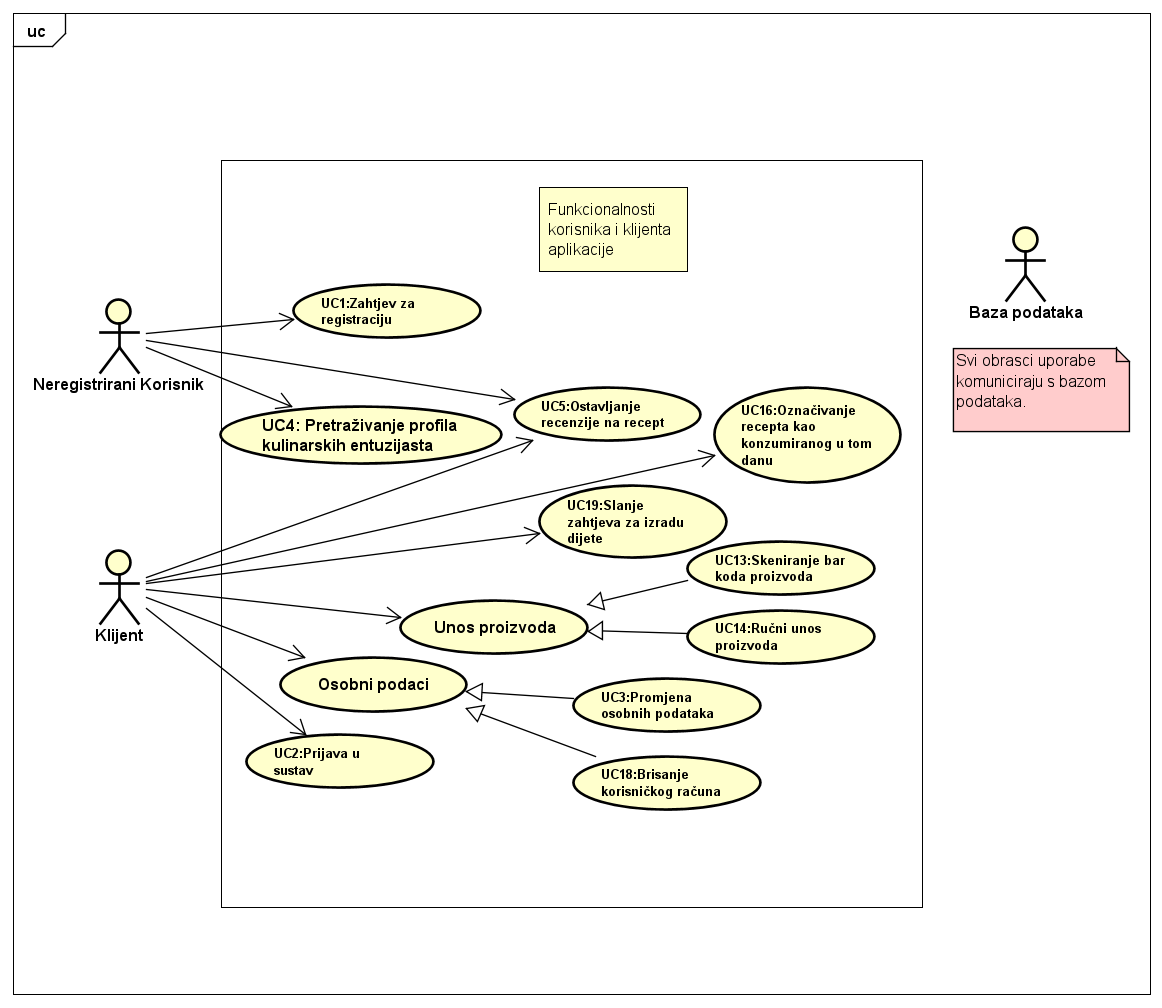
\includegraphics[scale=0.4]{dijagrami/UML_Korisnik_Klijent.png} %veličina slike u odnosu na originalnu datoteku i pozicija slike
			\centering
			\caption{Funkcionalnosti korisnika i klijenta aplikacije}
			\label{UML1}
		\end{figure}
		
		
				\begin{figure}[H]
			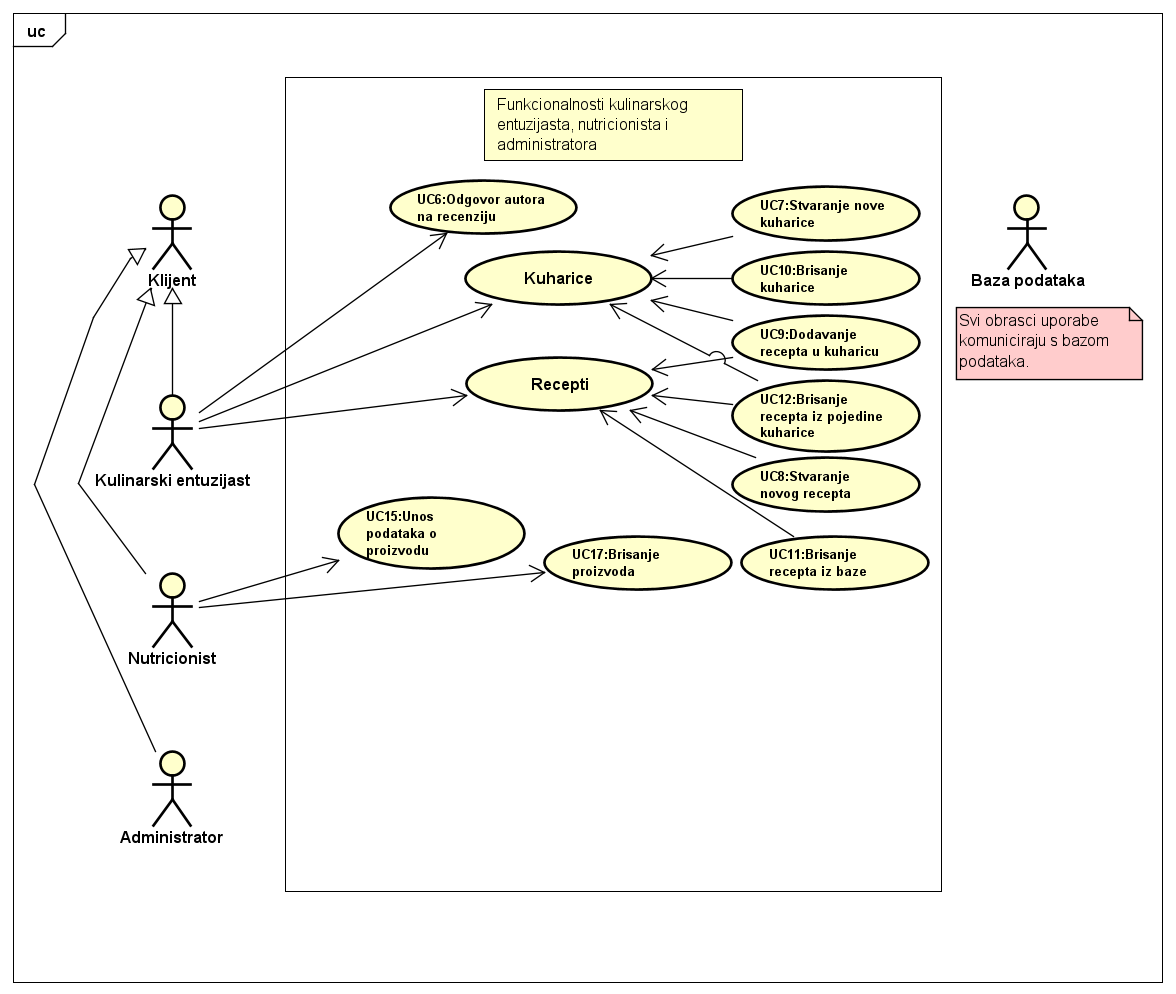
\includegraphics[scale=0.4]{dijagrami/UML_KulinarskiEntuzijast_Nutricionist_Admin.png} %veličina slike u odnosu na originalnu datoteku i pozicija slike
			\centering
			\caption{Funkcionalnosti kulinarskog entuzijasta, nutricionista i administratora aplikacije}
			\label{UML2}
		\end{figure}
				
			\subsection{Sekvencijski dijagrami}
				
				\begin{large}{\textbf{Obrazac uporabe UC4 - Pretraživanje profila kulinarskih entuzijasta}}\end{large}
				
				Korisnik šalje zahtjev za pretragom profila kulinarskih entuzijasta. Poslužitelj mu omogućava pristup i pretragu. Korisnik u tražilicu upisuje kategoriju po kojoj želi pretražiti kulinarske entuzijaste. Poslužitelj iz baze dohvaća sve kulinarske entuzijaste koji odgovaraju upisanoj kategoriji i prikazuje ih korisniku.
				
					
				\begin{figure}[H]
			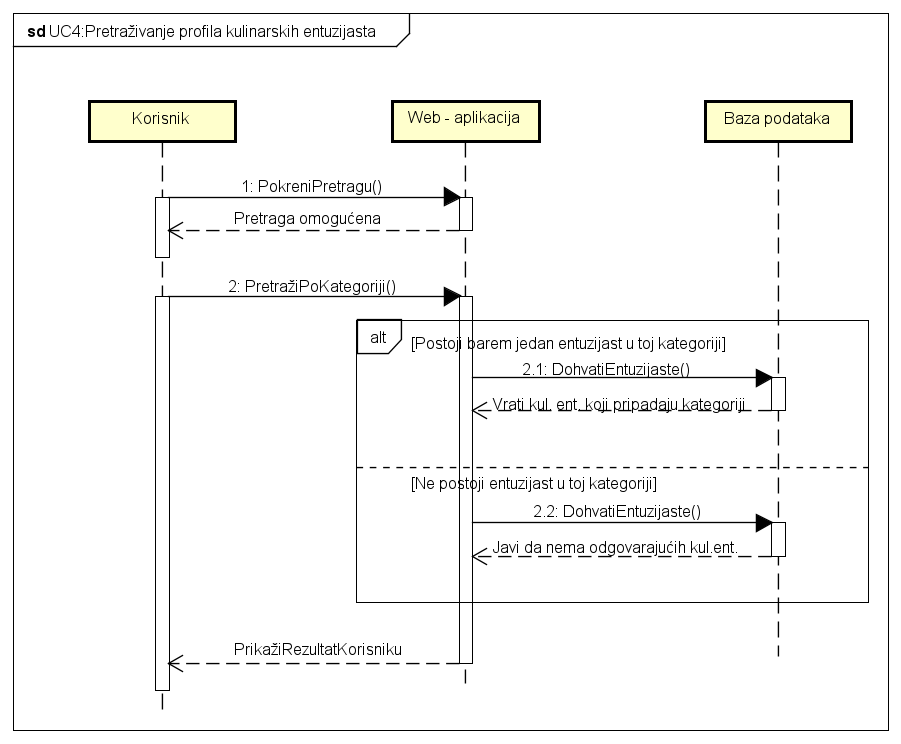
\includegraphics[scale=0.4]{dijagrami/SEQ_UC4.png} %veličina slike u odnosu na originalnu datoteku i pozicija slike
			\centering
			\caption{Sekvencijski dijagram za UC4}
			\label{SEQ_UC4}
		\end{figure}
	

				\begin{large}{\textbf{Obrazac uporabe UC8 - Stvaranje novog recepta}}\end{large}
				
				Kulinarski entuzijast šalje zahtjev za stvaranjem novog recepta. Poslužitelj mu omogućava pristup i stvaranje novog recepta. Kulinarski entuzijast upisuje sve podatke potrebne za stvaranje novog recepta: potrebne sastojke i njihovu količinu, korake pripreme, veličinu porcije, vrijeme kuhanja i galeriju popratnih slika. Nakon potvrde podataka, poslužitelj unosi novi recept u bazu podataka.
				
					
				\begin{figure}[H]
			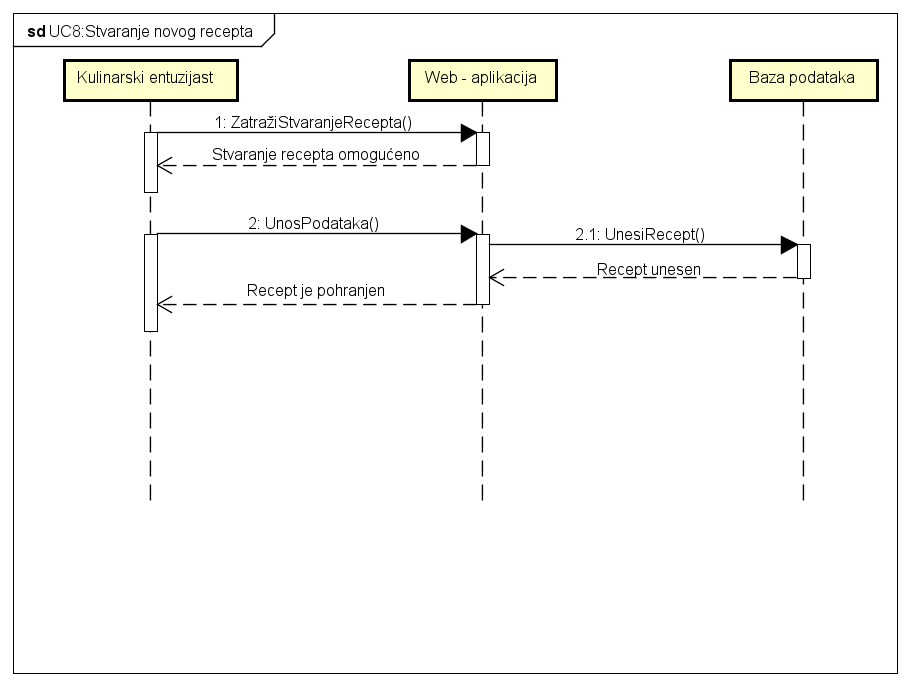
\includegraphics[scale=0.4]{dijagrami/SEQ_UC8.png} %veličina slike u odnosu na originalnu datoteku i pozicija slike
			\centering
			\caption{Sekvencijski dijagram za UC8}
			\label{SEQ_UC8}
		\end{figure}
				
			\begin{large}{\textbf{Obrazac uporabe UC13 - Skeniranje bar koda proizvoda}}\end{large}

			Klijent šalje zahtjev za skeniranjem bar koda proizvoda kojeg ima doma. Poslužitelj mu omogućava pristup i skeniranje bar koda proizvoda. Klijent skenira bar kod proizvoda, i ako je bar kod čitljiv i proizvod prepoznat, poslužitelj unosi skenirani proizvod u bazu podataka.
				
					
				\begin{figure}[H]
			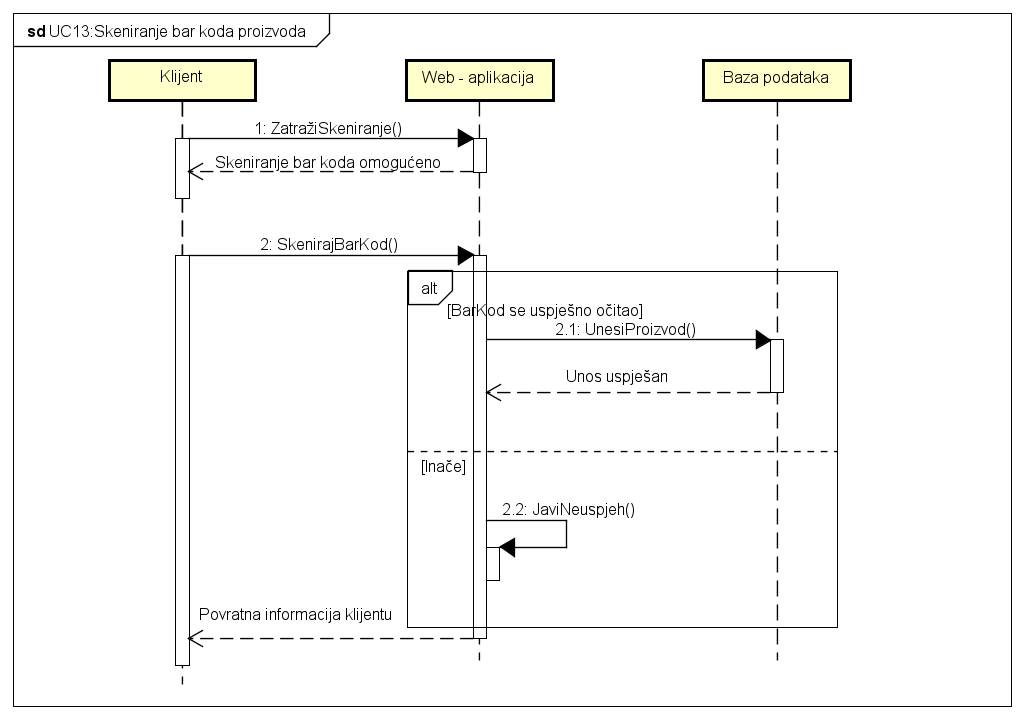
\includegraphics[scale=0.4]{dijagrami/SEQ_UC13.png} %veličina slike u odnosu na originalnu datoteku i pozicija slike
			\centering
			\caption{Sekvencijski dijagram za UC13}
			\label{SEQ_UC13}
		\end{figure}
				
			\begin{large}{\textbf{Obrazac uporabe UC14 - Ručni unos proizvoda}}\end{large}
			
			Klijent šalje zahtjev za ručnim unosom proizvoda kojeg ima doma. Poslužitelj mu omogućava pristup i unos proizvoda. Klijent unosi podatke o proizvodu ručno, primjerice njegov naziv, naziv proizvođača, masu, energetsku vrijednost itd. Nakon potvrde unosa, poslužitelj unosi novi recept u bazu podataka.
				
					
				\begin{figure}[H]
			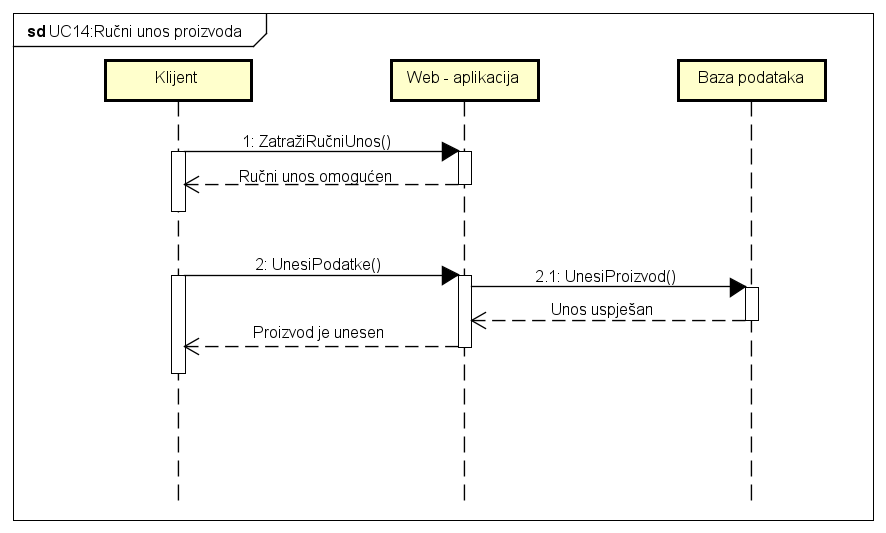
\includegraphics[scale=0.4]{dijagrami/SEQ_UC14.png} %veličina slike u odnosu na originalnu datoteku i pozicija slike
			\centering
			\caption{Sekvencijski dijagram za UC14}
			\label{SEQ_UC14}
		\end{figure}

		\section{Ostali zahtjevi}

			\begin{itemize}
			\item Sustav treba podržavati rad više korisnika u stvarnom vremenu.
			\item Sustav treba implementirati kao web aplikaciju koristeći objektno-orijentirane jezike.
			\item Sustav mora biti prilagođena veličini ekrana na kojem je prikazana.
			\item Sustav mora biti u potpunosti responzivan, bez dugog čekanja na podatke.
			\item Sustav mora biti što jednostavniji i prilagođeniji korisniku za korištenje.
			\item Sustav mora podržavati znakove hrvatske abecede pri unosu i prikazu sadržaja.
			\item Sustav mora imati omogućen pristup iz javne mreže.
			\item Sustav mora biti otporan na neispravno korištenje korisničkog sučelja, u smislu da neispravno korištenje ne smije narušiti njegovu funkcionalnost.
			\item Sustav mora ograničiti korisnika na pristup jedino onim resursima kojima ima pristup.
			\end{itemize}

			 
			 
	